%-------------------------------------------------------------------
% Unit Circle
%-------------------------------------------------------------------
\begin{Exercise}[title={Unit Circle},label=exUnitCircle]
	\Question Find the radian measure of the angle with the given degree measurements. 
	\begin{tasks}(2)
		\task 	 \ang{36}%$\frac{\pi }{5} \approx 0.628 \mbox{rad}$ 
		\task 	 \ang{-480}%$\frac{ -8 \pi }{3} \approx  -8.378 \mbox{rad}$
		\task 	 \ang{60}%$\frac{\pi }{3} \approx 1.047 \mbox{rad}$ 
		\task 	 \ang{-135}%$\frac{ -3 \pi }{4} \approx  -2.356 \mbox{rad}$
	\end{tasks}
\Question Find the degree measure of the angle with the given radian measure.  
\begin{tasks}(2)
	\task 	$\frac{3 \pi }{4}$ %\ang{135}
	\task 	$\frac{5 \pi }{6}$ %\ang{150}
	\task 	$ -1.5$ %$\frac{ -270}{\pi } \approx  \ang{-85.9}$
	\task 	$ -\frac{\pi }{12}$ %\ang{-15}
\end{tasks}
	\clearpage\Question Arc length
\begin{tasks}(2)
	\task 	 Find the length of the arc $s$ in the figure. The radius is $5$.\\%$\frac{55 \pi }{9} \approx 19.2$
	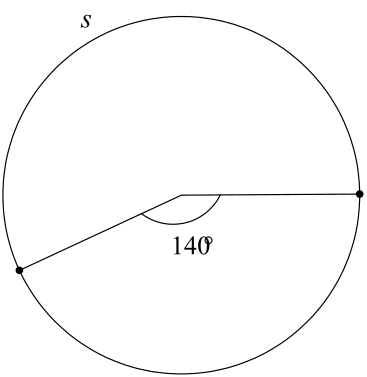
\includegraphics[width=4cm]{L4SZ281B}
	\task 	Find the radius $r$ of the circle in the figure. \\%$4$
	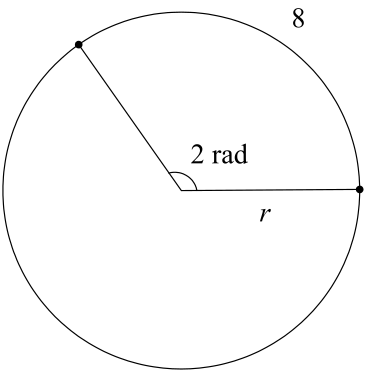
\includegraphics[width=4cm]{L4SZ281C}
\end{tasks}
	\Question Find the length of an arc that subtends a central angle of $2 \mbox{rad}$ in a circle of radius 2mi.%$4 \mbox{mi}$
	\Question Find the radius of the circle if an arc of length $6 \mbox{m}$ on the circle subtends a central angle of $\pi /6$ rad. %$\frac{36}{\pi } \approx 11.459 \mbox{m}$
	\Question Pittsburgh, Pennsylvania and Miami, Florida lie approximately on the same meridian. Pittsburgh has a latitude of $40.5 \mbox{{\ensuremath{{}^\circ}}}$ N and Miami is $25.5 \mbox{{\ensuremath{{}^\circ}}}$ N. Find the distance between these two cities. (The
radius of the earth is $3960 \mbox{mi}\text{.}$) %$330 \pi  \approx 1037 \mbox{mi}$
	\Question Find the distance the earth travels in one day in its path around the sun. Assume the year has $365$ days and that the path of the earth around the sun is a circle of radius $93$ million miles.%$1.6$ million $\mbox{mi}$
\end{Exercise}%unit circle
%---------------------------------------------
%--ANSWERS----UNIT CIRCLE---------------------
%---------------------------------------------
 \setboolean{firstanswerofthechapter}{true}
 \begin{Answer}[ref={exUnitCircle}]
\Question %Find the radian measure of the angle with the given degree measurements. 
\begin{tasks}
	\task 	 $\frac{\pi }{5} \approx 0.628 \mbox{rad}$ 
	\task 	 $\frac{ -8 \pi }{3} \approx  -8.378 \mbox{rad}$
	\task 	 $\frac{\pi }{3} \approx 1.047 \mbox{rad}$ 
	\task 	 $\frac{ -3 \pi }{4} \approx  -2.356 \mbox{rad}$
\end{tasks}
\Question %Find the degree measure of the angle with the given radian measure.  
\begin{tasks}
	\task 	\ang{135}
	\task 	\ang{150}
	\task 	$\frac{ -270}{\pi } \approx  \ang{-85.9}$
	\task 	\ang{-15}
\end{tasks}
\Question %Arc length
\begin{tasks}
	\task 	 $\frac{55 \pi }{9} \approx 19.2$
	\task 	$4$
\end{tasks}
\Question $4 \mbox{mi}$
\Question $\frac{36}{\pi } \approx 11.459 \mbox{m}$
\Question $330 \pi  \approx 1037 \mbox{mi}$
\Question $1.6$ million $\mbox{mi}$
\end{Answer}
\setboolean{firstanswerofthechapter}{false}
%-------------------------------------------------------------------
% Right Angled Trianges
%-------------------------------------------------------------------
\begin{Exercise}[title={Right Angled Triangles},label=exRightAngledTriangles]
	\Question Find the exact value of $\sin  \theta $, $\cos  \theta $ and $\tan  \theta $ of the angle $\theta $ in the triangle.%$\sin  \theta  =\frac{4}{5} ,\cos  \theta  =\frac{3}{5} ,\tan  \theta  =\frac{4}{3}$
	\Question Find $\sin  \theta $, $\cos  \theta $ and $\tan  \theta $ in the following triangles.
	
\begin{tasks}(2)
	\task 	 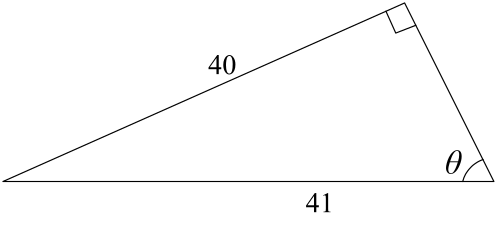
\includegraphics[ width=4cm]{L4SZ281L}%$\sin  \theta  =\frac{40}{41} ,\cos  \theta  =\frac{9}{41} ,\tan  \theta  =\frac{40}{9}$
	\task 	 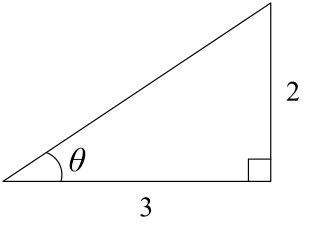
\includegraphics[ width=4cm]{L4SZ281M}%$\sin  \theta  =\frac{2 \sqrt{13}}{13} ,\cos  \theta  =\frac{3 \sqrt{13}}{13} ,\tan  \theta  =\frac{2}{3}$
\end{tasks}

\Question Find the side length labelled $x$ for the following triangles.
\begin{tasks}(3)
	\task 	 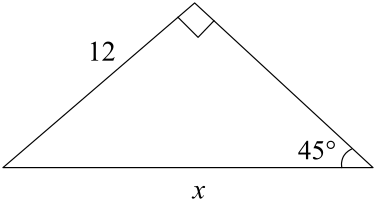
\includegraphics[ width=3.5cm]{L4SZ281N}%$12 \sqrt{2}$
	\task 	 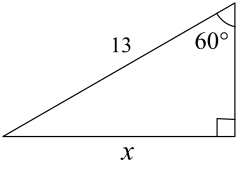
\includegraphics[ width=3.5cm]{L4SZ281O}%$\frac{13 \sqrt{3}}{2}$ 
	\task 	 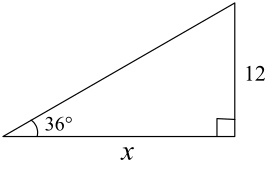
\includegraphics[ width=3.5cm]{L4SZ281P}%$16.51658$ 	
\end{tasks}

\clearpage	\Question Solve the triangles.
\begin{tasks}(2)
	\task 	 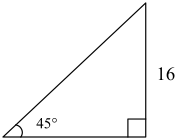
\includegraphics[ width=4.5cm]{L4SZ281Q}%$45 \mbox{{\ensuremath{{}^\circ}}} ,16 ,16 \sqrt{2} \approx 22.63$
	\task 	 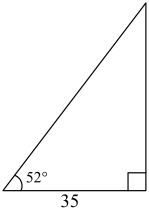
\includegraphics[ width=3cm]{L4SZ281R}%$38 \mbox{{\ensuremath{{}^\circ}}} ,44.79 ,56.85$ 
\end{tasks}

\Question The angle of elevation to the top of the Empire State Building in New York is found to be $11 \mbox{{\ensuremath{{}^\circ}}}$ from the ground at a distance of $1 \mbox{mi}$ from the base of the building. Using this information,
find the height of the Empire State Building.%$1026 \mbox{ft}$
	
	\Question A laser beam is to be directed towards the centre of the moon but the beam strays $0.5 \mbox{{\ensuremath{{}^\circ}}}$ from its intended path.
\begin{tasks}
	\task 	How far has the beam diverged from its assigned target when it reaches the moon? (The distance of the earth	to the moon is $240$ $000 \mbox{mi}\text{.}$) %$2100 \mbox{mi}$	
	\task 	The radius of the moon is about $1000 \mbox{mi}$. Will the beam strike the moon? %No
\end{tasks}

\Question A water tower is located $325 \mbox{ft}$ from a building. From a window in the building it is observed that the angle of elevation to the top of the tower is $39 \mbox{{\ensuremath{{}^\circ}}}$ and the angle of depression to the bottom of the tower is $25 \mbox{{\ensuremath{{}^\circ}}}$. How tall is the tower? How high is the window? %$415 \mbox{ft} ,152 \mbox{ft}$
\Question Find the area of a triangle with sides of length $7$ and $9$ and included angle $72 \mbox{{\ensuremath{{}^\circ}}}$.%30.0 
\Question A triangle has an area of $16 in^{2}\text{,}$ and two of the sides of the triangle have lengths $5 \mbox{in}$ and $7 \mbox{in}$. Find the angle included by these two sides.%\ang{66.1}

\end{Exercise}%right triangles
%---------------------------------------------
%--ANSWERS----RIGHT TRIANGLES-----------------
%---------------------------------------------
\begin{Answer}[ref={exRightAngledTriangles}]

\Question %Find the exact value of $\sin  \theta $, $\cos  \theta $ and $\tan  \theta $ of the angle $\theta $ in the triangle.
$\sin  \theta  =\frac{4}{5} ,\cos  \theta  =\frac{3}{5} ,\tan  \theta  =\frac{4}{3}$
\Question %Find $\sin  \theta $, $\cos  \theta $ and $\tan  \theta $ in the following triangles.

\begin{tasks}
	\task 	 $\sin  \theta  =\frac{40}{41} ,\cos  \theta  =\frac{9}{41} ,\tan  \theta  =\frac{40}{9}$
	\task 	 $\sin  \theta  =\frac{2 \sqrt{13}}{13} ,\cos  \theta  =\frac{3 \sqrt{13}}{13} ,\tan  \theta  =\frac{2}{3}$
\end{tasks}

\Question %Find the side length labelled $x$ for the following triangles.
\begin{tasks}
	\task 	 $12 \sqrt{2}$
	\task 	 $\frac{13 \sqrt{3}}{2}$ 
	\task 	 $16.51658$ 	
\end{tasks}

\Question %Solve the triangles.
\begin{tasks}
	\task 	 $45 \mbox{{\ensuremath{{}^\circ}}} ,16 ,16 \sqrt{2} \approx 22.63$
	\task 	 $38 \mbox{{\ensuremath{{}^\circ}}} ,44.79 ,56.85$ 
\end{tasks}

\Question %Empire State Building in New York 
$1026 \mbox{ft}$

\Question %A laser beam is to be directed towards the centre of the moon 
\begin{tasks}
	\task 	$2100 \mbox{mi}$	
	\task 	No
\end{tasks}

\Question %A water tower is located $325 \mbox{ft}$ from a building.
$415 \mbox{ft} ,152 \mbox{ft}$
\Question 30.0 
\Question \ang{66.1}

\end{Answer}%RightAngledTriangles

%-------------------------------------------------------------------
% Trigonometric Functions
%-------------------------------------------------------------------
\begin{Exercise}[title={Trigonometric Functions},label=exTrigonometricFunctions]
	\Question Sketch the functions by hand. 
	\begin{tasks}(2)
		\task 	 $y =1 +\sin  x$ %soln file {L4SZ270N}
		\task 	 $y =1 -\cos  x$ %soln file {L4SZ270O}
		\task 	 $y = -2 \sin  x$ %soln file {L4SZ270P}
		\task 	 $y =4 -2 \cos  x$%soln file  {L4SZ270Q}
		\task 	 $y =\left \vert \cos  x\right \vert $%soln file {L4SZ270R}
	\end{tasks}
	\Question Find the amplitude and period of the function and sketch its graph. 
	\begin{tasks}(2)
		\task 	$y =\cos  4 x$  %soln file {L4SZ270S} $1 ,\frac{\pi }{2}$
		\task 	$y =3 \sin  3 x$  %soln file {L4SZ270T} $3 ,\frac{2 \pi }{3}$
		\task 	$y =10 \sin  \frac{1}{2} x$ %soln file {L4SZ270U} $10 ,4 \pi $
		\task 	$y = -\cos  \frac{1}{3} x$ %soln file {L4SZ270V} $1 ,6 \pi $
		\task   $y =3 \cos  3 \pi  x$%soln file {L4SZ270W} $3 ,\frac{2}{3}$
	\end{tasks}
	\Question Find the amplitude, period and phase shift of the function, and plot using \desmos. 
\begin{tasks}(2)
	\task 	$y =\cos  \left (x -\frac{\pi }{2}\right )$  %soln file {L4SZ270X} $1 ,2 \pi  ,\frac{\pi }{2}$
	\task 	$y = -\sin  \left (x -\frac{\pi }{6}\right )$  %soln file {L4SZ270Y} $2 ,2 \pi  ,\frac{\pi }{6}$
	\task 	$y =2 \sin  \left (\frac{2}{3} x -\frac{\pi }{6}\right )$  %soln file {L4SZ2710} $2 ,3 \pi  ,\frac{\pi }{4}$
	\task 	$y =3 \cos  \pi  \left (x +\frac{1}{2}\right )$ %soln file {L4SZ2711} $3 ,2 , -\frac{1}{2}$
	\task   $y = -\frac{1}{2} \cos  \left (2 x -\frac{\pi }{3}\right )$ %soln file {L4SZ2712}  $\frac{1}{2} ,\pi  ,\frac{\pi }{6}$
	\task	$y =\sin  \left (3 x +\pi \right )$%soln file {L4SZ2713} $1 ,\frac{2 \pi }{3} , -\frac{\pi }{3}$
\end{tasks}
\end{Exercise}%Trigonometric Functions
%---------------------------------------------
%--ANSWERS----TRIG FUNCTIONS------------------
%---------------------------------------------
\begin{Answer}[ref={exTrigonometricFunctions}]

	\Question %Sketch the functions by hand. 
\begin{tasks}
	\task 	 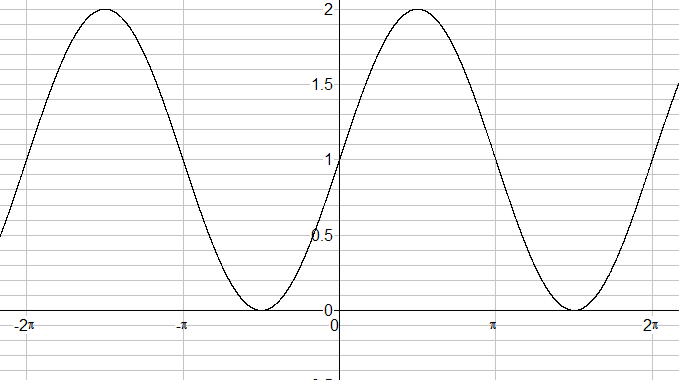
\includegraphics[width=4cm]{L4SZ270N}
	\task 	 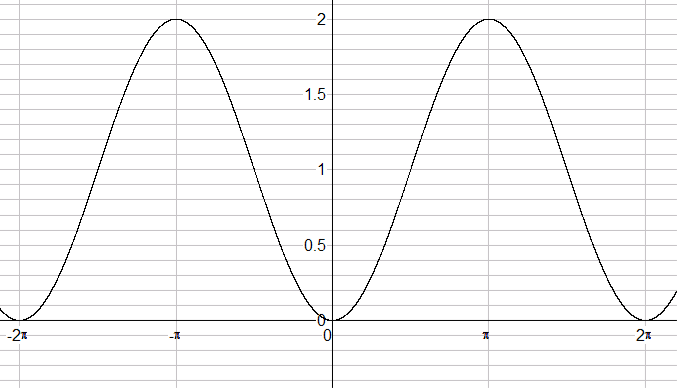
\includegraphics[width=4cm]{L4SZ270O}
	\task 	 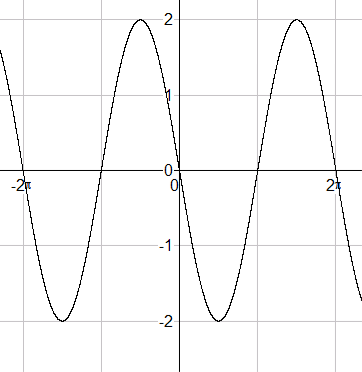
\includegraphics[width=4cm]{L4SZ270P}
	\task 	 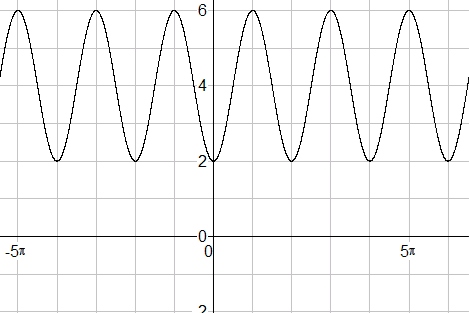
\includegraphics[width=4cm]{L4SZ270Q}
	\task 	 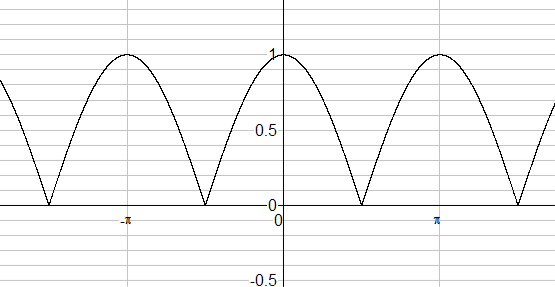
\includegraphics[width=4cm]{L4SZ270R}
\end{tasks}
\Question %Find the amplitude and period of the function and sketch its graph. 
\begin{tasks}
	\task 	$1 ,\frac{\pi }{2}$\\	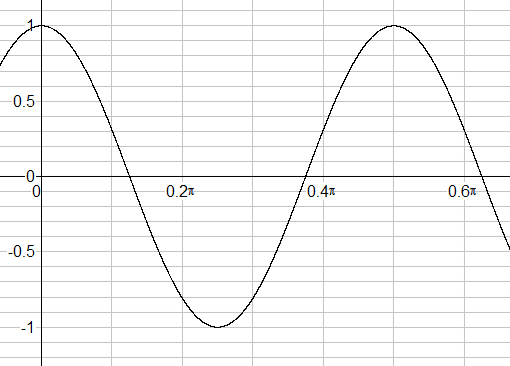
\includegraphics[width=4cm]{L4SZ270S}
	\task 	$3 ,\frac{2 \pi }{3}$\\	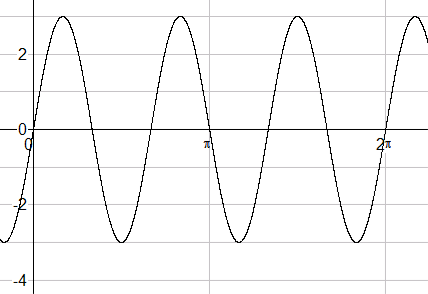
\includegraphics[width=4cm]{L4SZ270T}
	\task 	$10 ,4 \pi $\\			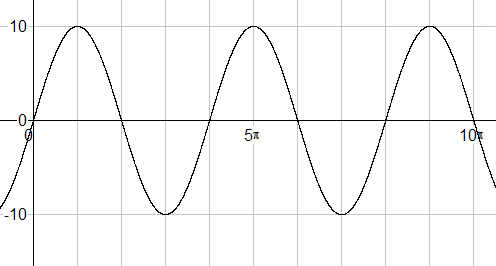
\includegraphics[width=4cm]{L4SZ270U} 
	\task 	$1 ,6 \pi $\\			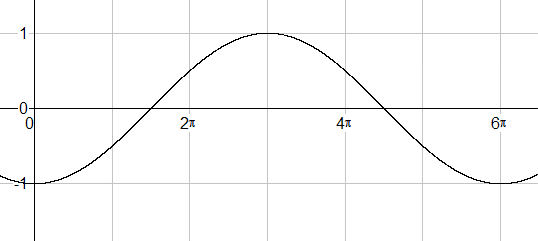
\includegraphics[width=4cm]{L4SZ270V} 
	\task   $3 ,\frac{2}{3}$\\		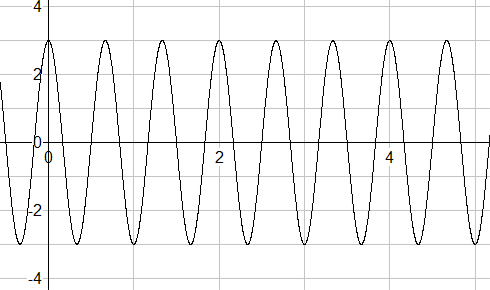
\includegraphics[width=4cm]{L4SZ270W} 
\end{tasks}
\Question %Find the amplitude, period and phase shift of the function, and plot using \desmos. 
\begin{tasks}
	\task 	$1 ,2 \pi  ,\frac{\pi }{2}$\\ 	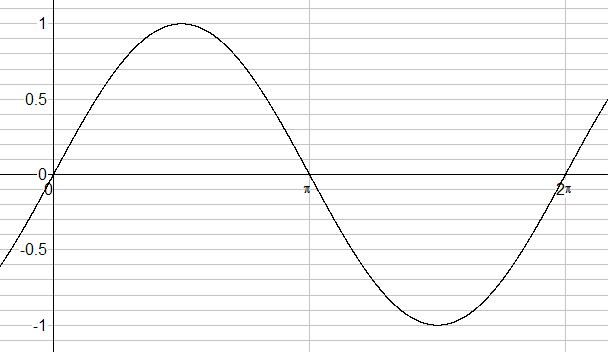
\includegraphics[width=4cm]{L4SZ270X} 
	\task 	$2 ,2 \pi  ,\frac{\pi }{6}$\\	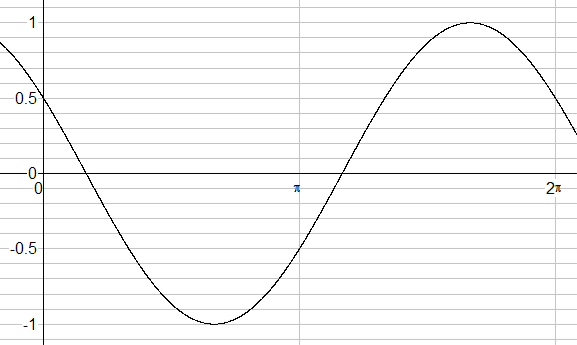
\includegraphics[width=4cm]{L4SZ270Y} 
	\task 	$2 ,3 \pi  ,\frac{\pi }{4}$\\	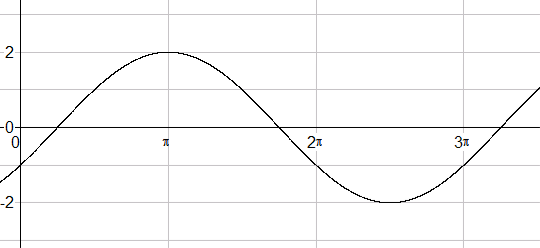
\includegraphics[width=4cm]{L4SZ2710} 
	\task 	$3 ,2 , -\frac{1}{2}$\\			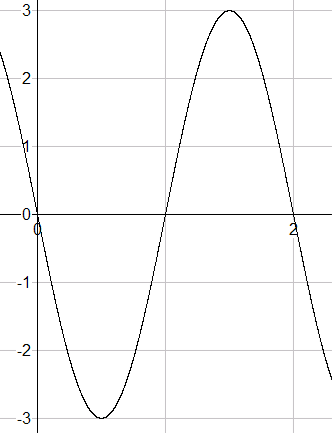
\includegraphics[width=4cm]{L4SZ2711} 
	\task   $\frac{1}{2} ,\pi  ,\frac{\pi }{6}$\\		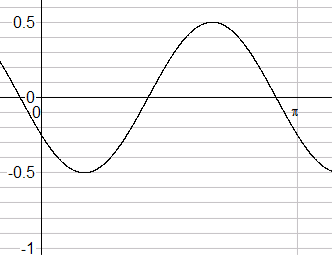
\includegraphics[width=4cm]{L4SZ2712}  
	\task	$1 ,\frac{2 \pi }{3} , -\frac{\pi }{3}$\\	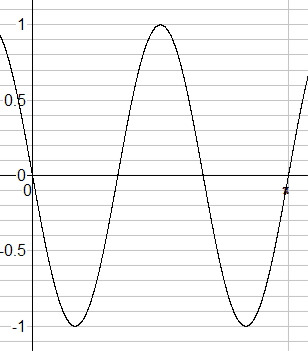
\includegraphics[width=4cm]{L4SZ2713} 
\end{tasks}

\end{Answer}%TrigonometricFunctions

%-------------------------------------------------------------------
% Applications
%-------------------------------------------------------------------
\begin{Exercise}[title={Applications},label=exApplications]
	\Question Use the Sine Rule to find side $x$ or angle $\theta $ 
	\begin{tasks}(2)
		\task 	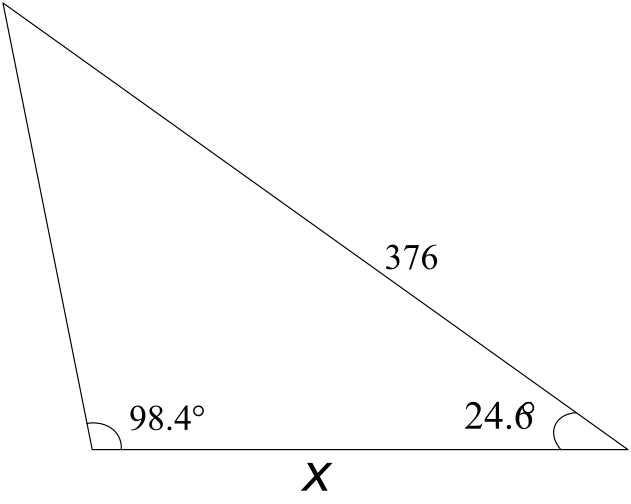
\includegraphics[width=4cm]{L4SZ2823}%$318.8$ 
		\task 	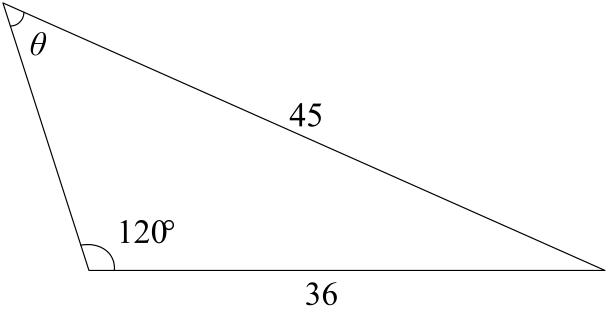
\includegraphics[width=4cm]{L4SZ2824}%	\ang{44}
	\end{tasks}
	\Question Solve the triangle using the Sine Rule.  \\
	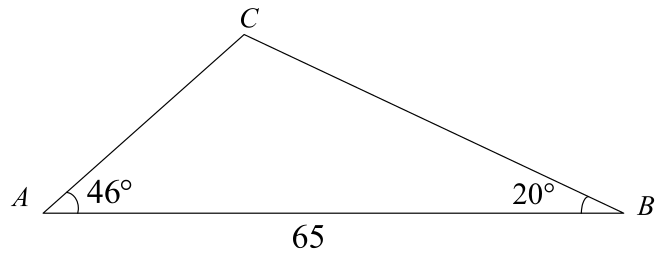
\includegraphics[width=4cm]{L4SZ2825}%	$\angle C =114 \mbox{{\ensuremath{{}^\circ}}} ,a \approx 51 ,b \approx 24$
		\Question Sketch each triangle and then solve using the Sine Rule. 
	\begin{tasks}(2)
		\task 	$\angle A =50 \mbox{{\ensuremath{{}^\circ}}}\text{,}$ $\angle B =68 \mbox{{\ensuremath{{}^\circ}}}\text{,}$ $c =230$% $\angle C =62 \mbox{{\ensuremath{{}^\circ}}} ,a \approx 200 b \approx 242$
		\task 	$\angle B =29 \mbox{{\ensuremath{{}^\circ}}}\text{,}$ $\angle C =51 \mbox{{\ensuremath{{}^\circ}}}\text{,}$ $b =44$%$\angle A =100 \mbox{{\ensuremath{{}^\circ}}} ,a \approx 89 ,c \approx 71$
	\end{tasks}
\begin{multicols}{2}
	\Question To find the distance across a river, a surveyor chooses points $A$ and $B$, which are $200 \mbox{ft}$ apart on one side of the river. She then chooses a reference point $C$ on the opposite side of the river and finds that $\angle BAC \approx 82 \mbox{{\ensuremath{{}^\circ}}}$ and $\angle ABC \approx 52 \mbox{{\ensuremath{{}^\circ}}}\text{.}$  Find the approximate distance from $A$ to $C$. \\%$219 \mbox{ft}$
	\columnbreak 
	
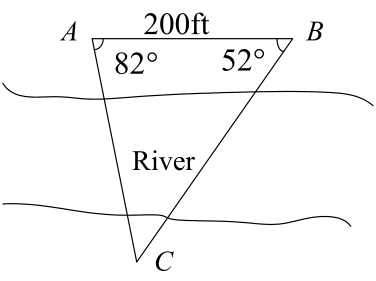
\includegraphics[width=4cm]{L4SZ2826}	\\
\end{multicols}

	\Question The path of a satellite circling the earth causes it to pass directly over two tracking stations $A$ and $B$, which are $50 \mbox{mi}$ apart. When the satellite is on one side of thetwo stations, the angle of elevation at $A$ and $B$ are measured to be $87.0 \mbox{{\ensuremath{{}^\circ}}}$ and $84.2 \mbox{{\ensuremath{{}^\circ}}}$, respectively.  
\begin{tasks}(2)
	\task How far is the satellite from	station $A$?%$1018 \mbox{mi}\text{,}$
	\task How high is the satellite	above the ground?%$1017 \mbox{mi}$
\end{tasks}
	
\begin{multicols}{2}
	\Question A communication tower is located at the top of a steep hill. The angle of inclination
	of the hill is $58 \mbox{{\ensuremath{{}^\circ}}}$. A guy wire is attached to the top of the tower and to the ground, $100 \mbox{m}$ downhill from the base of the tower. The angle between the slope of the hill and the guy wire is measured as $12 \mbox{{\ensuremath{{}^\circ}}}$. Find $A C$, the length of cable required for the guy wire. %$155 \mbox{m}$
	\columnbreak 
	
	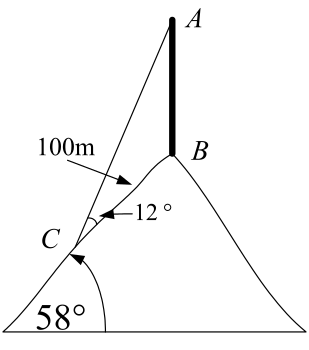
\includegraphics[width=4cm]{L4SZ2827}	\\
\end{multicols}	
	\clearpage\Question Use the Cosine Rule to find side $x$ given $AC=44.3$ and $\theta$. 
\begin{tasks}(2)
	\task 	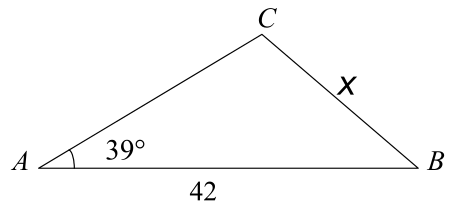
\includegraphics[width=5cm]{L4SZ282D}%28.9
	\task 	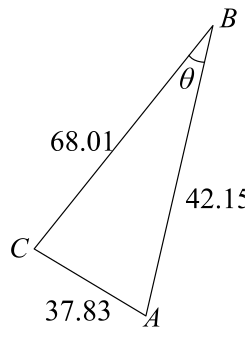
\includegraphics[width=3cm]{L4SZ282E}%\ang{28.89}
\end{tasks}
\Question Use either the Sine Rule or Cosine Rule as appropriate to find $x$ and $\theta$.
	\begin{tasks}(2)
		\task 	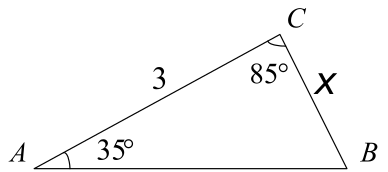
\includegraphics[width=4cm]{L4SZ282G}%2
		\task 	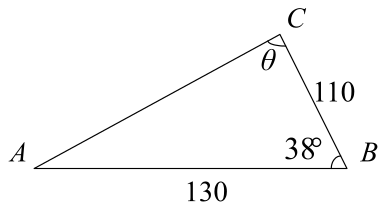
\includegraphics[width=4cm]{L4SZ282H}%\ang{84.6}
	\end{tasks}
\Question Two straight roads diverge at an angle of $65 \mbox{{\ensuremath{{}^\circ}}}$. Two cars leave the intersection at $2.00$ P.M., one traveling at $50 mi/\mbox{h}$ and the other at $30 mi/\mbox{h}$. How far apart are the cars at $2.30$ P.M.?%$23.1 \mbox{mi}$
\Question A pilot flies in a straight path for $1 \mbox{h}\; 30 \mbox{min}$. She then makes a course correction, heading $10 \mbox{{\ensuremath{{}^\circ}}}$ to the right of her original course, and flies for $2 \mbox{h}$ in the new direction. If she maintains a constant speed of $625 mi/\mbox{h}$ how far is she from her starting point?%$2179 \mbox{mi}$

\begin{multicols}{2}
	\Question A steep mountain is inclined $74 \mbox{{\ensuremath{{}^\circ}}}$ to the horizontal and rises $3400 \mbox{ft}$ above the surrounding plain. A cable car is to be installed from a point $800 \mbox{ft}$ from the base to the top of the mountain, as shown. Find the shortest length of cable needed.%$3835 \mbox{ft}$ 
	\columnbreak 
	
	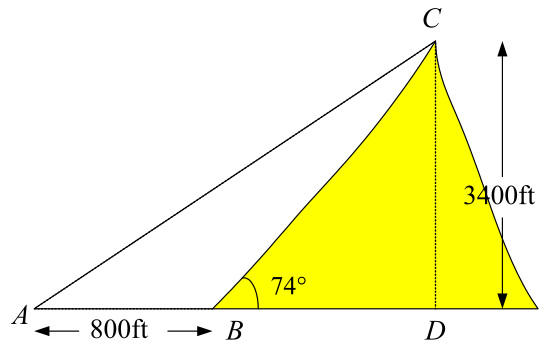
\includegraphics[width=6cm]{L4SZ282J}	\\
\end{multicols}	

\begin{multicols}{2}
	\Question Three circles of radii $4$, $5$, and $6 \mbox{cm}$ respectively are mutually tangent. Find the area enclosed between the circles.%$3.85 cm^{2}$
	\columnbreak 
	
	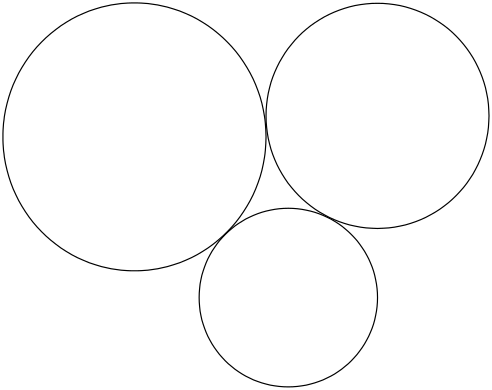
\includegraphics[width=6cm]{L4SZ282K}	\\
\end{multicols}	

\begin{multicols}{2}
	\Question A surveyor wishes to find the distance between two points $A$ and $B$ on the opposite side of a river. on her side of the river she chooses two points $C$ and $D$ that are $20 \mbox{m}$ apart and measures the angles shown. Find	the distance between $A$ and $B\text{.}$%$14.3 \mbox{m}$
	\columnbreak 
	
	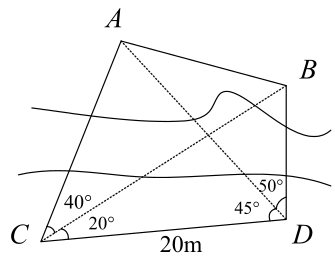
\includegraphics[width=6cm]{L4SZ282L}	\\
\end{multicols}	
%---------------------------------------------
%--ANSWERS----APPLICATIONS--------------------
%---------------------------------------------
\end{Exercise}%Applications
\begin{Answer}[ref={exApplications}]

	\Question %Use the Sine Rule to find side $x$ or angle $\theta $ 
\begin{tasks}
	\task 	$318.8$ 
	\task 	\ang{44}
\end{tasks}
\Question %Solve the triangle using the Sine Rule.
$\angle C =114 \mbox{{\ensuremath{{}^\circ}}} ,a \approx 51 ,b \approx 24$
\Question %Sketch each triangle and then solve using the Sine Rule. 
\begin{tasks}
	\task 	$\angle C =62 \mbox{{\ensuremath{{}^\circ}}} ,a \approx 200 b \approx 242$
	\task 	$\angle A =100 \mbox{{\ensuremath{{}^\circ}}} ,a \approx 89 ,c \approx 71$
\end{tasks}
	\Question% To find the distance across a river, a surveyor\\%
	$219 \mbox{ft}$

\Question %The path of a satellite circling the earth  
\begin{tasks}
	\task $1018 \mbox{mi}\text{,}$
	\task $1017 \mbox{mi}$
\end{tasks}

	\Question %A communication tower is located at the top of a steep hill. 
	$155 \mbox{m}$
	
\Question %Use the Cosine Rule to find side $x$ given $AC=44.3$ and $\theta$. 
\begin{tasks}
	\task 	28.9
	\task 	\ang{28.89}
\end{tasks}
\Question %Use either the Sine Rule or Cosine Rule as appropriate to find $x$ and $\theta$.
\begin{tasks}
	\task 	2
	\task 	\ang{84.6}
\end{tasks}
\Question %Two straight roads diverge at an angle 
$23.1 \mbox{mi}$
\Question %A pilot flies in a straight path 
$2179 \mbox{mi}$

	\Question %A steep mountain is inclined 
	$3835 \mbox{ft}$ 
	\Question %Three circles of radii 
	$3.85 cm^{2}$
	\Question %A surveyor wishes to find the distance between two points
	$14.3 \mbox{m}$
	
\end{Answer}%Applications

%-------------------------------------------------------------------
% END exercises
%-------------------------------------------------------------------

